% Options for packages loaded elsewhere
\PassOptionsToPackage{unicode}{hyperref}
\PassOptionsToPackage{hyphens}{url}
%
\documentclass[
  12pt,
]{article}
\usepackage{amsmath,amssymb}
\usepackage{iftex}
\ifPDFTeX
  \usepackage[T1]{fontenc}
  \usepackage[utf8]{inputenc}
  \usepackage{textcomp} % provide euro and other symbols
\else % if luatex or xetex
  \usepackage{unicode-math} % this also loads fontspec
  \defaultfontfeatures{Scale=MatchLowercase}
  \defaultfontfeatures[\rmfamily]{Ligatures=TeX,Scale=1}
\fi
\usepackage{lmodern}
\ifPDFTeX\else
  % xetex/luatex font selection
\fi
% Use upquote if available, for straight quotes in verbatim environments
\IfFileExists{upquote.sty}{\usepackage{upquote}}{}
\IfFileExists{microtype.sty}{% use microtype if available
  \usepackage[]{microtype}
  \UseMicrotypeSet[protrusion]{basicmath} % disable protrusion for tt fonts
}{}
\makeatletter
\@ifundefined{KOMAClassName}{% if non-KOMA class
  \IfFileExists{parskip.sty}{%
    \usepackage{parskip}
  }{% else
    \setlength{\parindent}{0pt}
    \setlength{\parskip}{6pt plus 2pt minus 1pt}}
}{% if KOMA class
  \KOMAoptions{parskip=half}}
\makeatother
\usepackage{xcolor}
\usepackage[margin=1in]{geometry}
\usepackage{graphicx}
\makeatletter
\def\maxwidth{\ifdim\Gin@nat@width>\linewidth\linewidth\else\Gin@nat@width\fi}
\def\maxheight{\ifdim\Gin@nat@height>\textheight\textheight\else\Gin@nat@height\fi}
\makeatother
% Scale images if necessary, so that they will not overflow the page
% margins by default, and it is still possible to overwrite the defaults
% using explicit options in \includegraphics[width, height, ...]{}
\setkeys{Gin}{width=\maxwidth,height=\maxheight,keepaspectratio}
% Set default figure placement to htbp
\makeatletter
\def\fps@figure{htbp}
\makeatother
\setlength{\emergencystretch}{3em} % prevent overfull lines
\providecommand{\tightlist}{%
  \setlength{\itemsep}{0pt}\setlength{\parskip}{0pt}}
\setcounter{secnumdepth}{5}
\usepackage{setspace} \usepackage{amsmath} \usepackage{array} \usepackage{caption} \usepackage{longtable} \usepackage{booktabs} \usepackage{enumitem} \renewcommand{\arraystretch}{1} \captionsetup[table]{skip=5pt} \setstretch{1.5}
\ifLuaTeX
  \usepackage{selnolig}  % disable illegal ligatures
\fi
\usepackage[]{natbib}
\bibliographystyle{apalike}
\IfFileExists{bookmark.sty}{\usepackage{bookmark}}{\usepackage{hyperref}}
\IfFileExists{xurl.sty}{\usepackage{xurl}}{} % add URL line breaks if available
\urlstyle{same}
\hypersetup{
  pdftitle={Experiment Results},
  pdfauthor={Zark Zijian Wang},
  hidelinks,
  pdfcreator={LaTeX via pandoc}}

\title{Experiment Results}
\author{Zark Zijian Wang}
\date{October 17, 2023}

\begin{document}
\maketitle

\hypertarget{experimental-procedure}{%
\section{Experimental Procedure}\label{experimental-procedure}}

In our survey, each question is a choice list. In each row of the list,
participants are required to choose between an immediate reward
(labelled as ``option A'') and a two-reward sequence (labelled as
``option B''). The two-reward sequence is constituted by an immediate
reward and a delayed reward. Every participant is presented with the
same questions.

There are two conditions in the survey. The first condition is called
``Immediate reward varies''. In each question of this condition, the
amount of the immediate reward in option B increases by £10 with each
row, starting from £10 and going up to £100, while the other variables
keep constant. The second condition is called ``Delayed reward varies''.
In the second condition, the amount of the delayed reward in option B
varies across the rows, following the same pattern as the first
condition, while the others keep constant. For each condition, the
reward amount of option A is selected from \{£120, £100\}, the reward
constant across rows in option B is selected from \{£90, £70, £50\}. The
time length of option B, e.g.~when the delayed reward is delivered, is
selected from \{18 months, 9 months, 1 month\} for the first condition
and is 3 months for the second condition.

\hypertarget{data}{%
\section{Data}\label{data}}

160 participants were recruited via Prolific. All the participants are
British residents. 50\% of them are female, and the median age is 41. On
average, it took around 11.6 minutes for participants to finish the
survey, with nine tenths of the participants finishing within 20
minutes. Each participants received £2 after completing the survey. 157
participants passed attention check.

\hypertarget{descriptive-statistics}{%
\section{Descriptive Statistics}\label{descriptive-statistics}}

Standard deviation

\begin{figure}
  \centering
  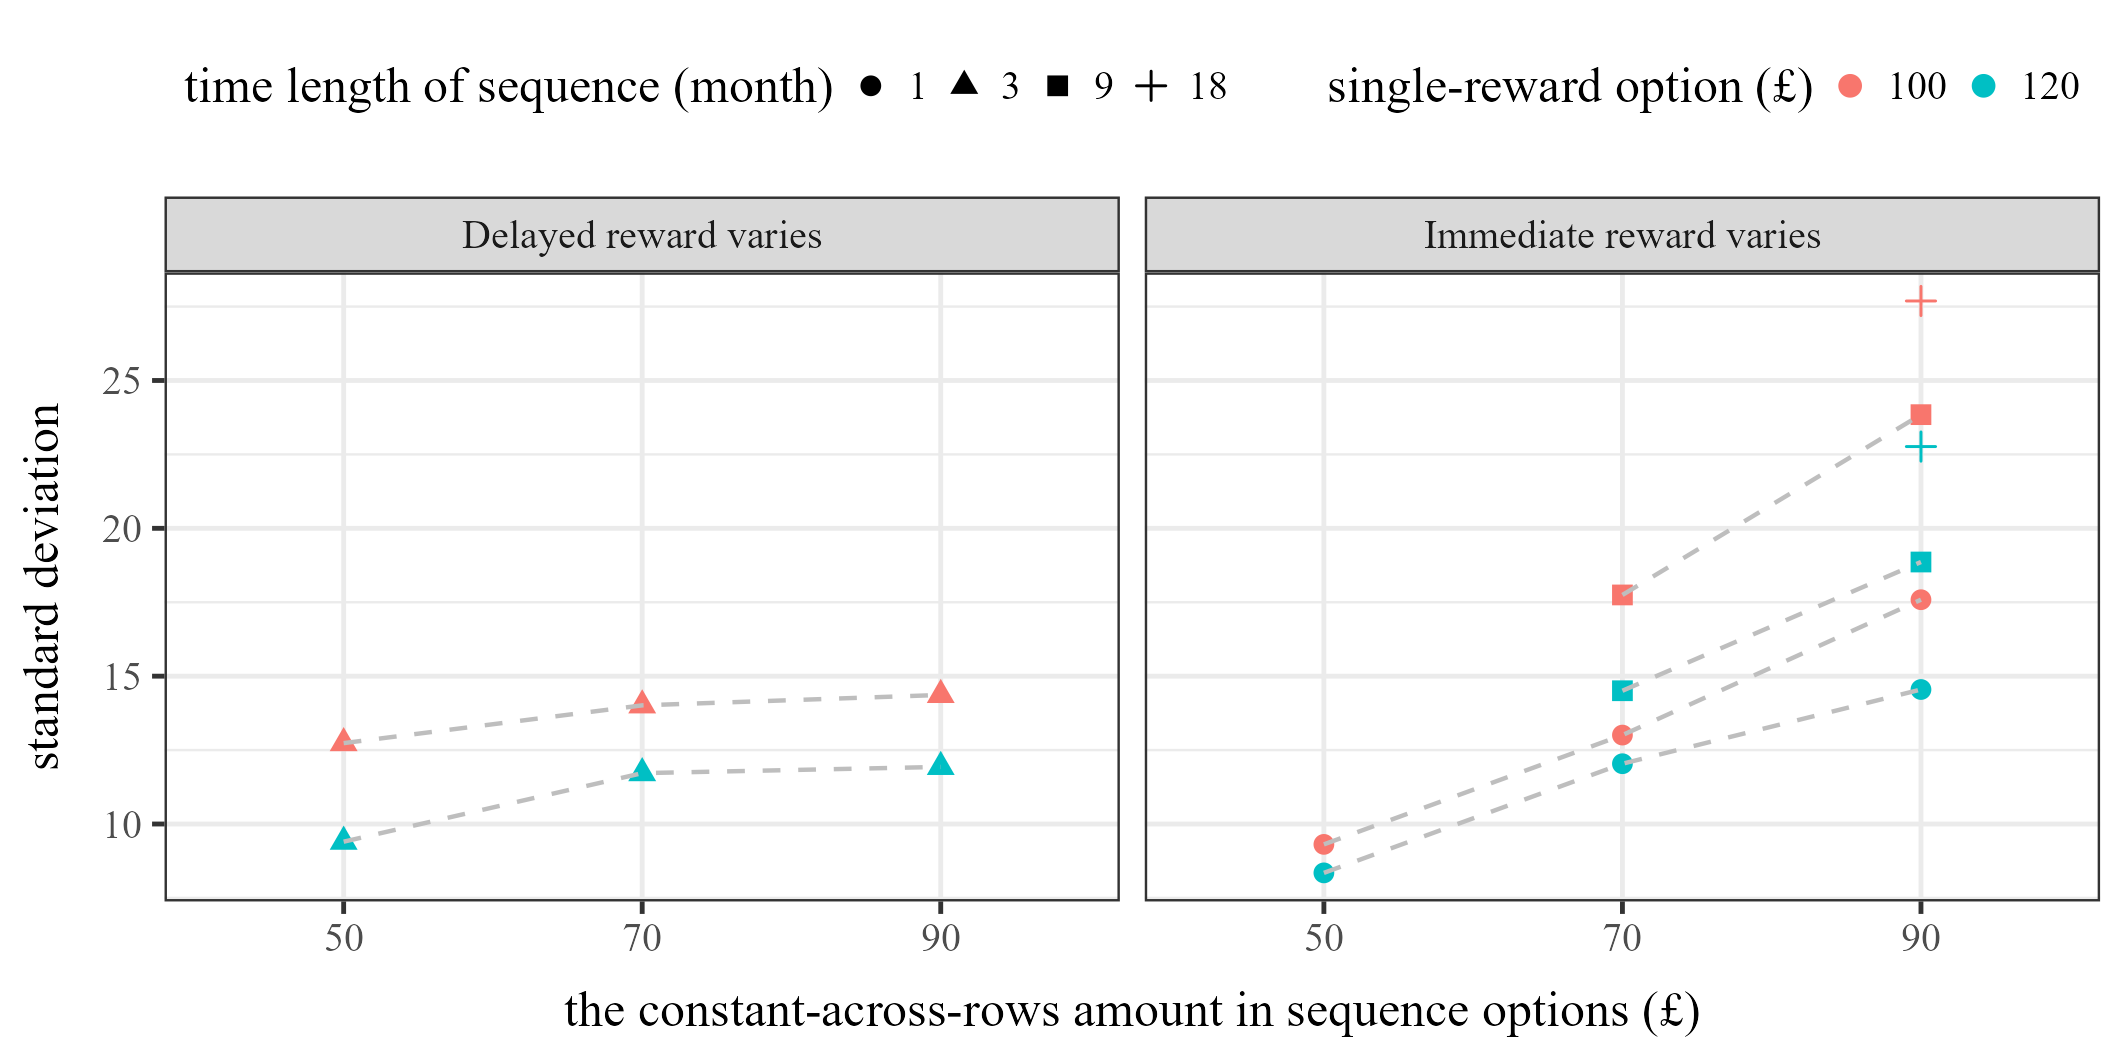
\includegraphics[width=0.96\textwidth]{figures/fig_switch_sd.png}
  \caption{Standard deviation of the swtich points in each question}
  \label{fig:choice-sd}
\end{figure}

\hypertarget{regression-analysis}{%
\section{Regression Analysis}\label{regression-analysis}}

\hypertarget{baseline-model}{%
\subsection{Baseline Model}\label{baseline-model}}

\hypertarget{utility-models}{%
\subsection{Utility Models}\label{utility-models}}

\begin{figure}
  \centering
  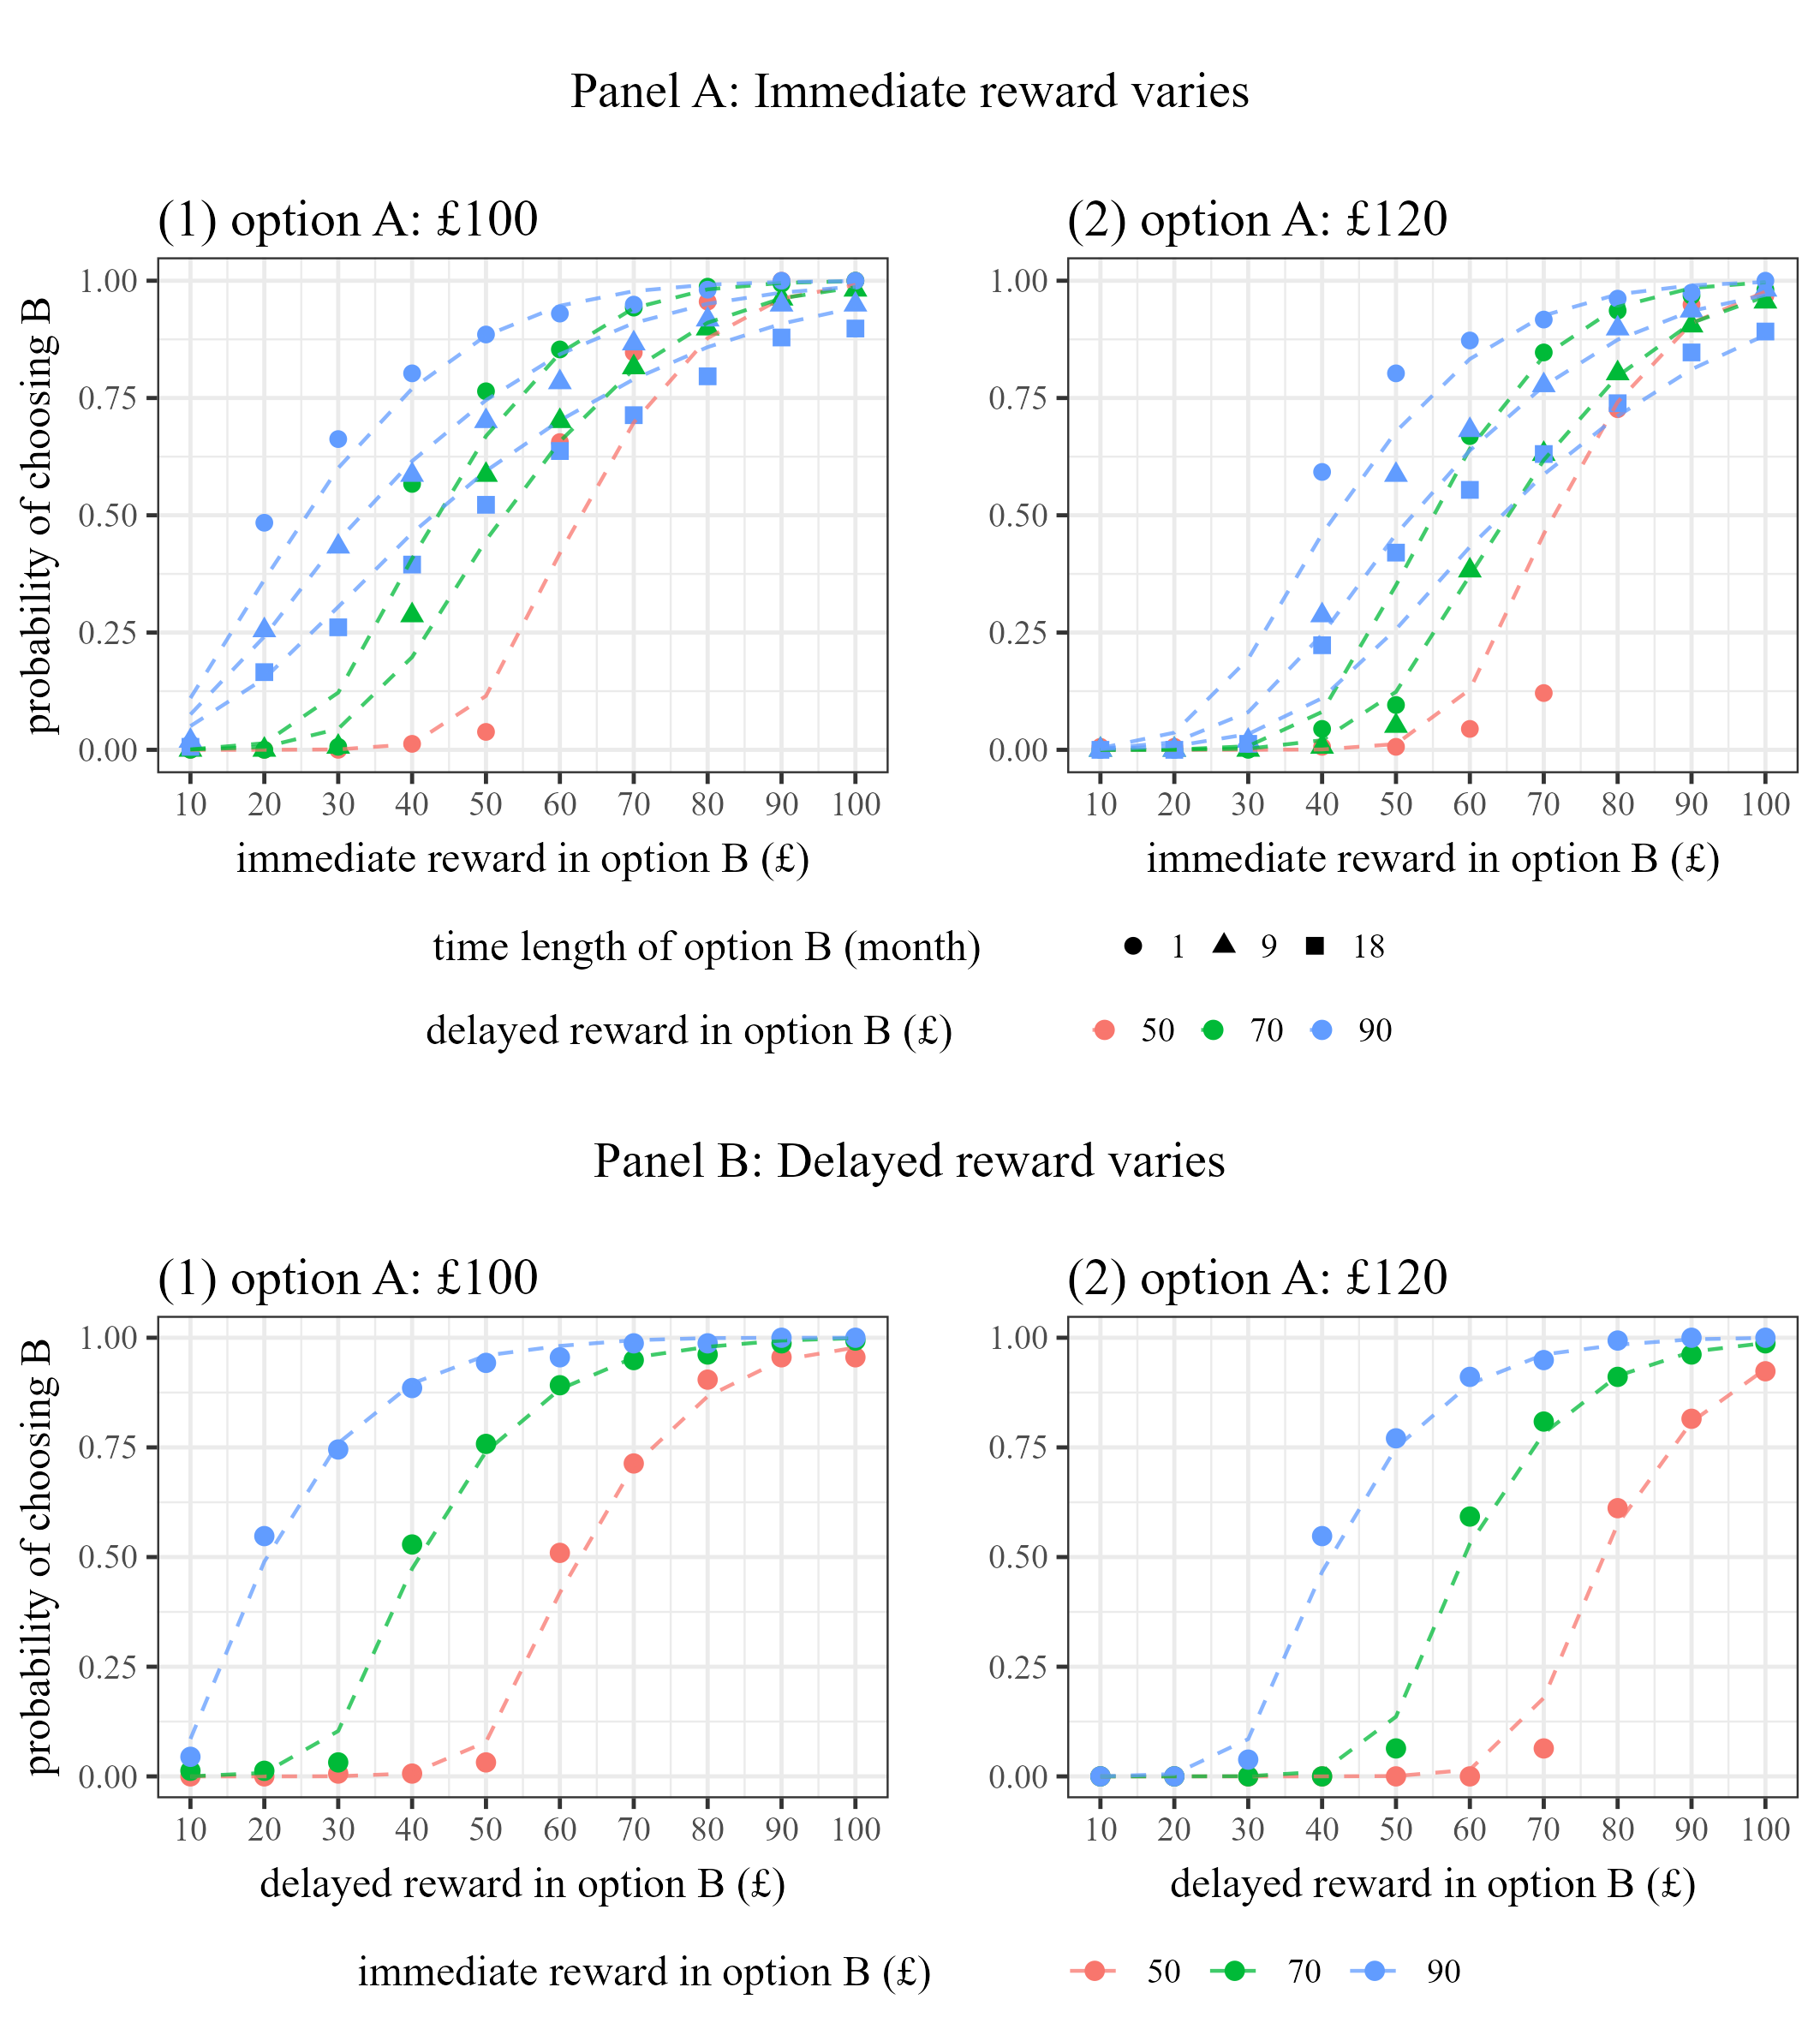
\includegraphics[width=0.96\textwidth]{figures/fig_grand_pred.png}
  \caption{Data and model predicted choice probabilities.}
  \caption*{\small Dots are the propotions of participants choosing option B in the data, dashed curves are the mean predicted choice probabilities for option B. The curves are fitted by a logit model on the censored data, with $X_v$ being transformed to $u(X_v)$, $M$ being added into interaction terms.}
  \label{fig:choice-predicted}
\end{figure}

\hypertarget{discussion}{%
\section{Discussion}\label{discussion}}

\end{document}
